\documentclass[border=0.5mm]{standalone}

\usepackage{import}
\subimport{../../../}{preamble.tex}

\usepackage{tikz}
\usetikzlibrary{calc}

\usepackage{pgfplots}
\usepgfplotslibrary{fillbetween}

\begin{document}

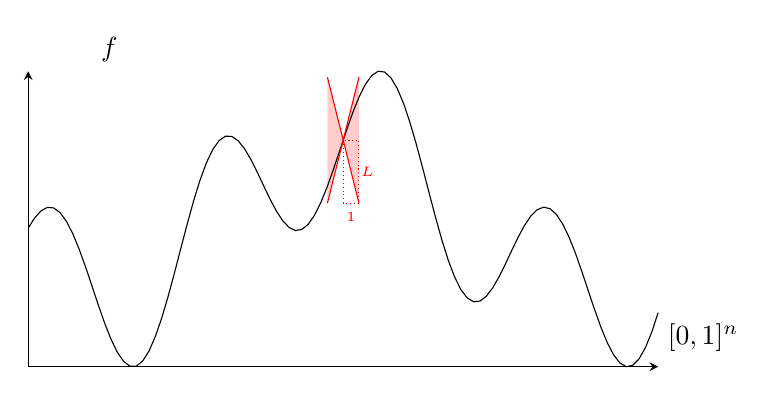
\begin{tikzpicture}

  \begin{axis}[
    ticks=none,
    axis lines=left,
    y=1cm,            % y unit vector
    x=1cm,            % x unit vector
    clip=false,
    xlabel={$[0, 1]^n$},
    ylabel={$f$},
    x label style={at={(axis description cs:1.0,0.1)},anchor=west},
    y label style={at={(axis description cs:0.1,1.0)},rotate=-90,anchor=south west},
    ]
    
    \addplot[mark=none, black, samples=100, domain=-4:4] {sin(3*360*x/(2*pi))+cos(360*x/(2*pi))};

    \addplot[name path=up, mark=none, red, samples=100, domain=-0.2:0.2] {1+4*x};
    \addplot[name path=down, mark=none, red, samples=100, domain=-0.2:0.2] {1-4*x};
    \addplot[red!20] fill between[
    of = up and down
    ];

    \draw[red, densely dotted] (axis cs:0,1) rectangle (axis cs:0.2,0.2);
    \node[red, below] at (axis cs:0.1,0.2) {\tiny $1$};
    \node[red, right] at (axis cs:0.1,0.6) {\tiny $L$};
    
    
  \end{axis}

  
\end{tikzpicture}

\end{document}

%%% Local Variables:
%%% mode: latex
%%% TeX-master: t
%%% End:
